
\documentclass[a4paper,12pt]{article}

\usepackage[utf8]{inputenc}
\usepackage[T1]{fontenc}
\usepackage{graphicx}
\usepackage{float}
\usepackage{geometry}

\geometry{margin=2.5cm}

\begin{document}

% =========================================================
% TITLE PAGE
% =========================================================

\begin{titlepage}

\newgeometry{top=1.5cm,bottom=1.5cm,left=2cm,right=2cm}

\begin{center}

\vspace*{0.5cm}

{\Large\textbf{ME-R-SY}}

\vspace{0.1cm}

{\small\textit{Meteorological Reporting System}}

\vspace{0.8cm}

\noindent\rule{0.85\textwidth}{1.2pt}

\vspace{1.0cm}

{\Huge\textbf{Rapport météorologique mensuel}}

\vspace{0.3cm}

{\Large
Analyse des conditions météorologiques\\
et des anomalies climatiques
}

\vspace{0.8cm}

% =========================================================
% MAIN FIGURE
% =========================================================

\includegraphics[
    width=0.82\textwidth,
    height=7cm,
    keepaspectratio
]{figures/mean\_2018\_01.png}

\vspace{0.3cm}

{\small\textit{Distribution spatiale des conditions météorologiques
au Maroc}}

\vspace{0.8cm}

% =========================================================
% PERIOD
% =========================================================

\fbox{%
\begin{minipage}{0.55\textwidth}
\centering
\vspace{0.25cm}

{\large\textbf{Période étudiée}}

\vspace{0.1cm}

{\LARGE\textbf{01 / 2018}}

\vspace{0.15cm}

{\small Référence climatique : 1991--2020}

\vspace{0.25cm}
\end{minipage}
}

\vfill

% =========================================================
% DESCRIPTION
% =========================================================

\begin{minipage}{0.80\textwidth}
\centering
\small
Rapport généré automatiquement à partir des données
météorologiques et des analyses statistiques du système ME-R-SY.
\end{minipage}

\vspace{0.8cm}

\noindent\rule{0.85\textwidth}{0.6pt}

\vspace{0.25cm}

{\small
\textbf{ME-R-SY}
\quad | \quad
Meteorological Data Analysis
\quad | \quad
Automated Reporting
}

\end{center}

\restoregeometry

\end{titlepage}


\section{Synthèse générale}

Pour le mois de janvier 2018, comparé à la période de référence 1991-2020, les analyses mettent en évidence les anomalies et extrêmes météorologiques suivants :

Concernant la température à 2 mètres (t2m), l'anomalie globale du mois s'établit à +0,41 °C. La température maximale journalière a atteint 33,63 °C le 30 janvier 2018 à 15:00 UTC à la position (22,0°N, -3,25°W). À l'opposé, la température minimale a descendu à 1

\begin{figure}[H]
    \centering
    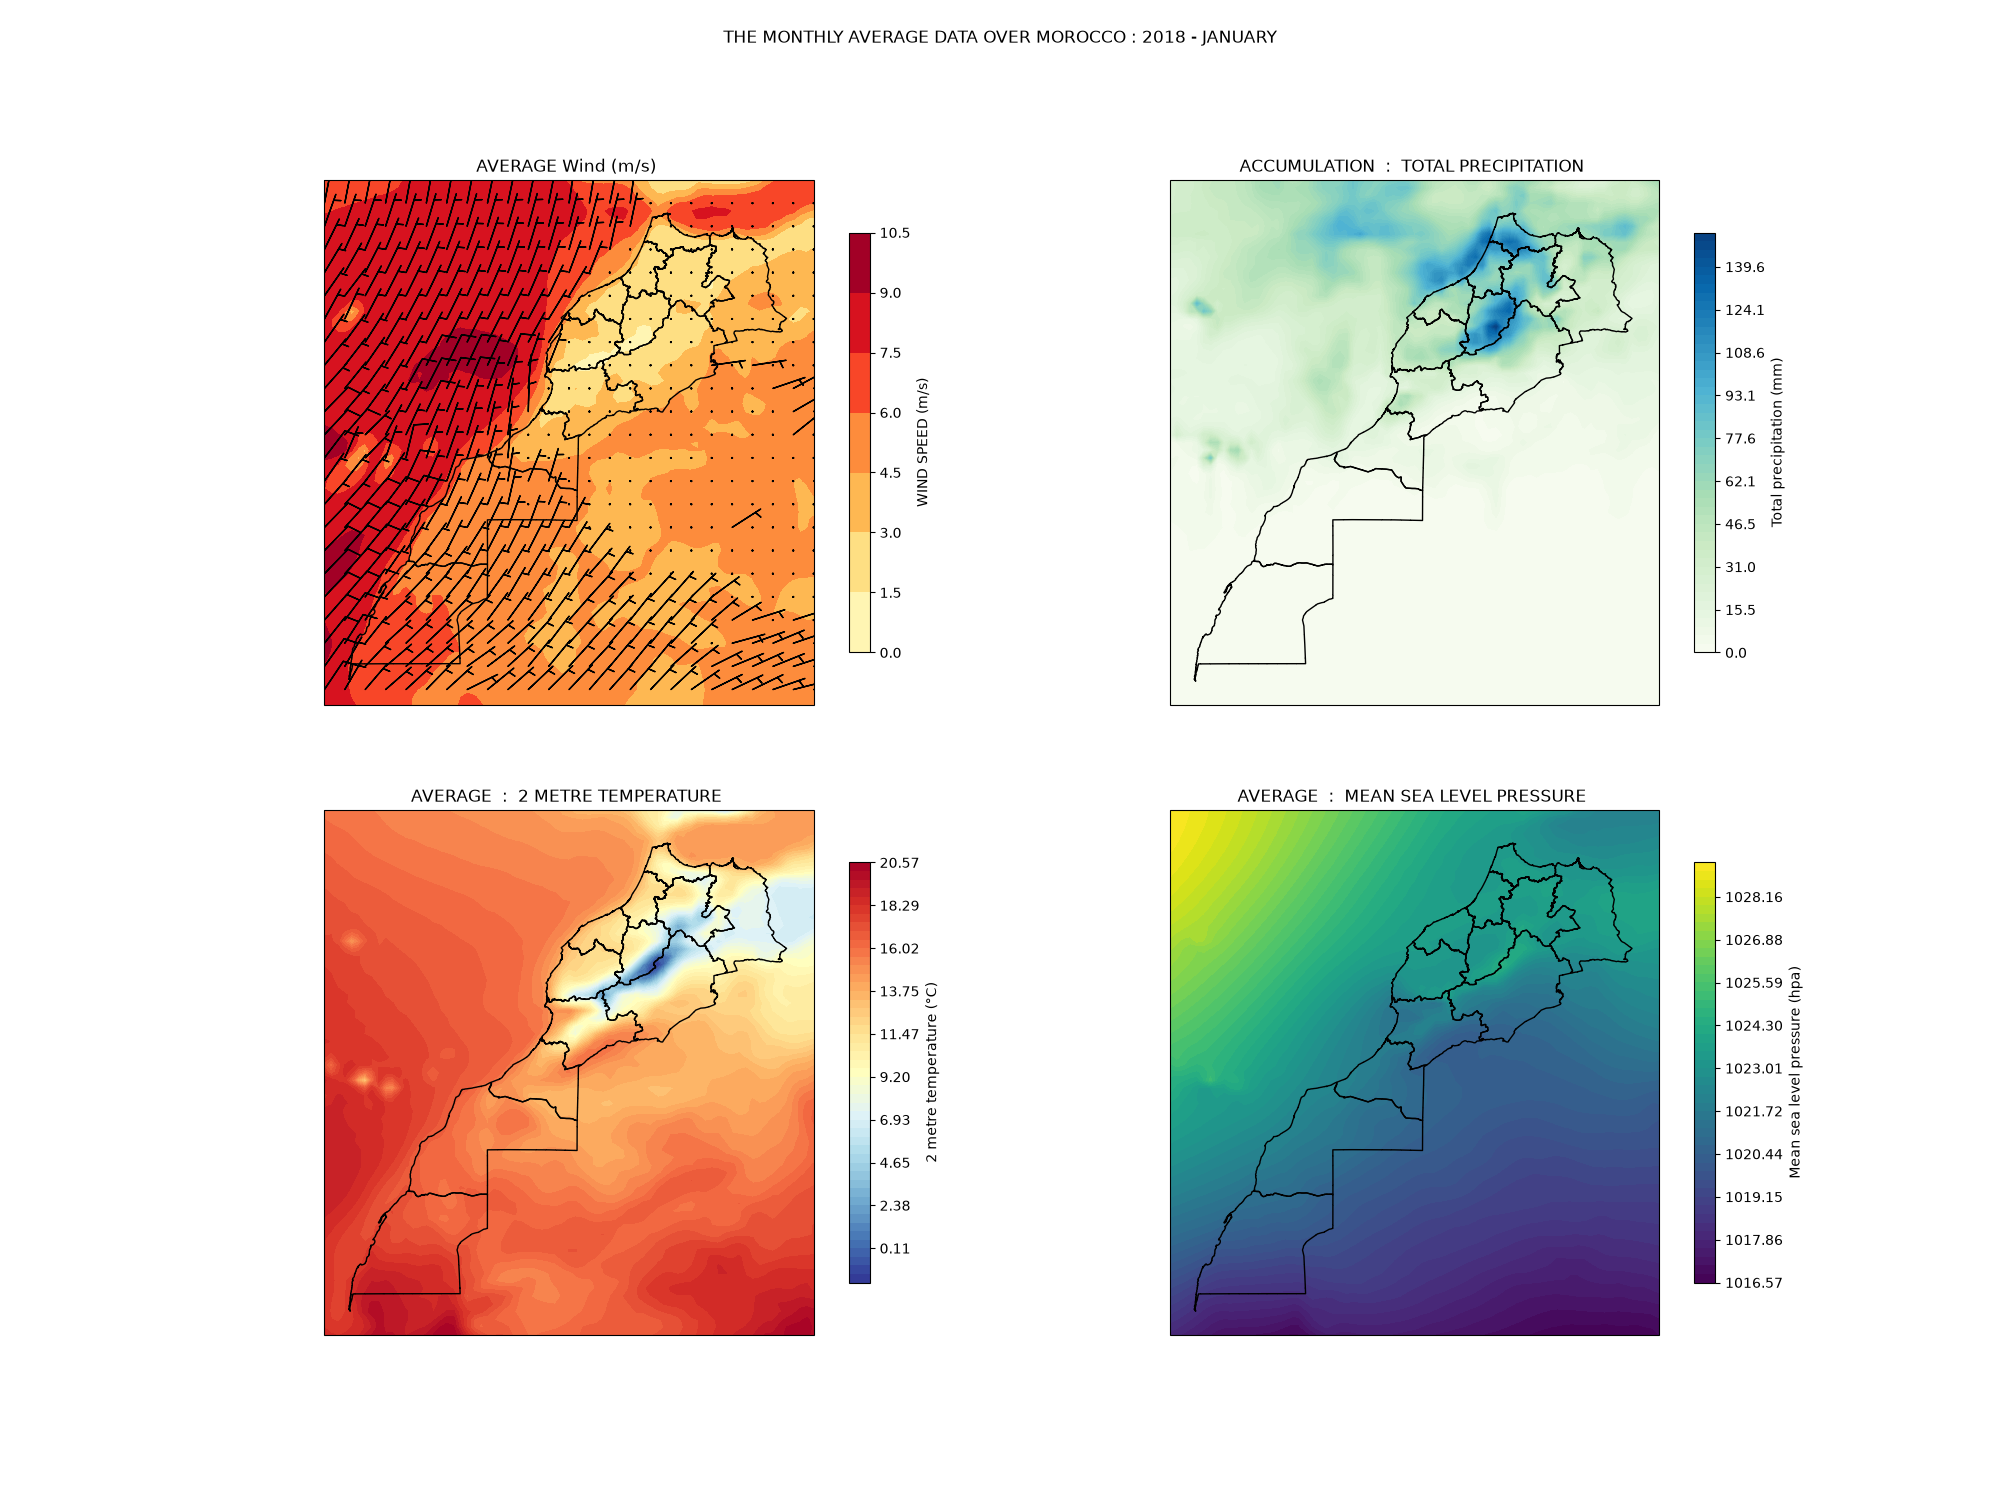
\includegraphics[width=\textwidth]{figures/mean_2018_01.png}
    \caption{Moyennes météorologiques}
\end{figure}

\section{Conditions mensuelles}

Pour le mois de janvier 2018, l'analyse météorologique met en évidence les extrêmes et anomalies suivants par rapport à la période de référence (1991-2020) :

Concernant la température à 2 mètres (t2m), la valeur maximale enregistrée est de 33,63 °C le 30 janvier 2018 à 15:00 UTC à la position (22,0°N, -3,25°O). La température minimale s'ét

\section{Maximums}

Durant le mois de janvier 2018, la température maximale de l'air à 2 mètres a atteint 33,63 °C le 30 janvier à 15:00 UTC, localisée par 22,0°N et -3,25°O. Concernant la dynamique atmosphérique de surface, la composante zonale du vent (u10) a enregistré un maximum de 15,93 m/s le 6 janvier à 18:00 UTC (35,75°N, -3,0°O), tandis que la composante méridienne (v10) a culminé à

\begin{figure}[H]
    \centering
    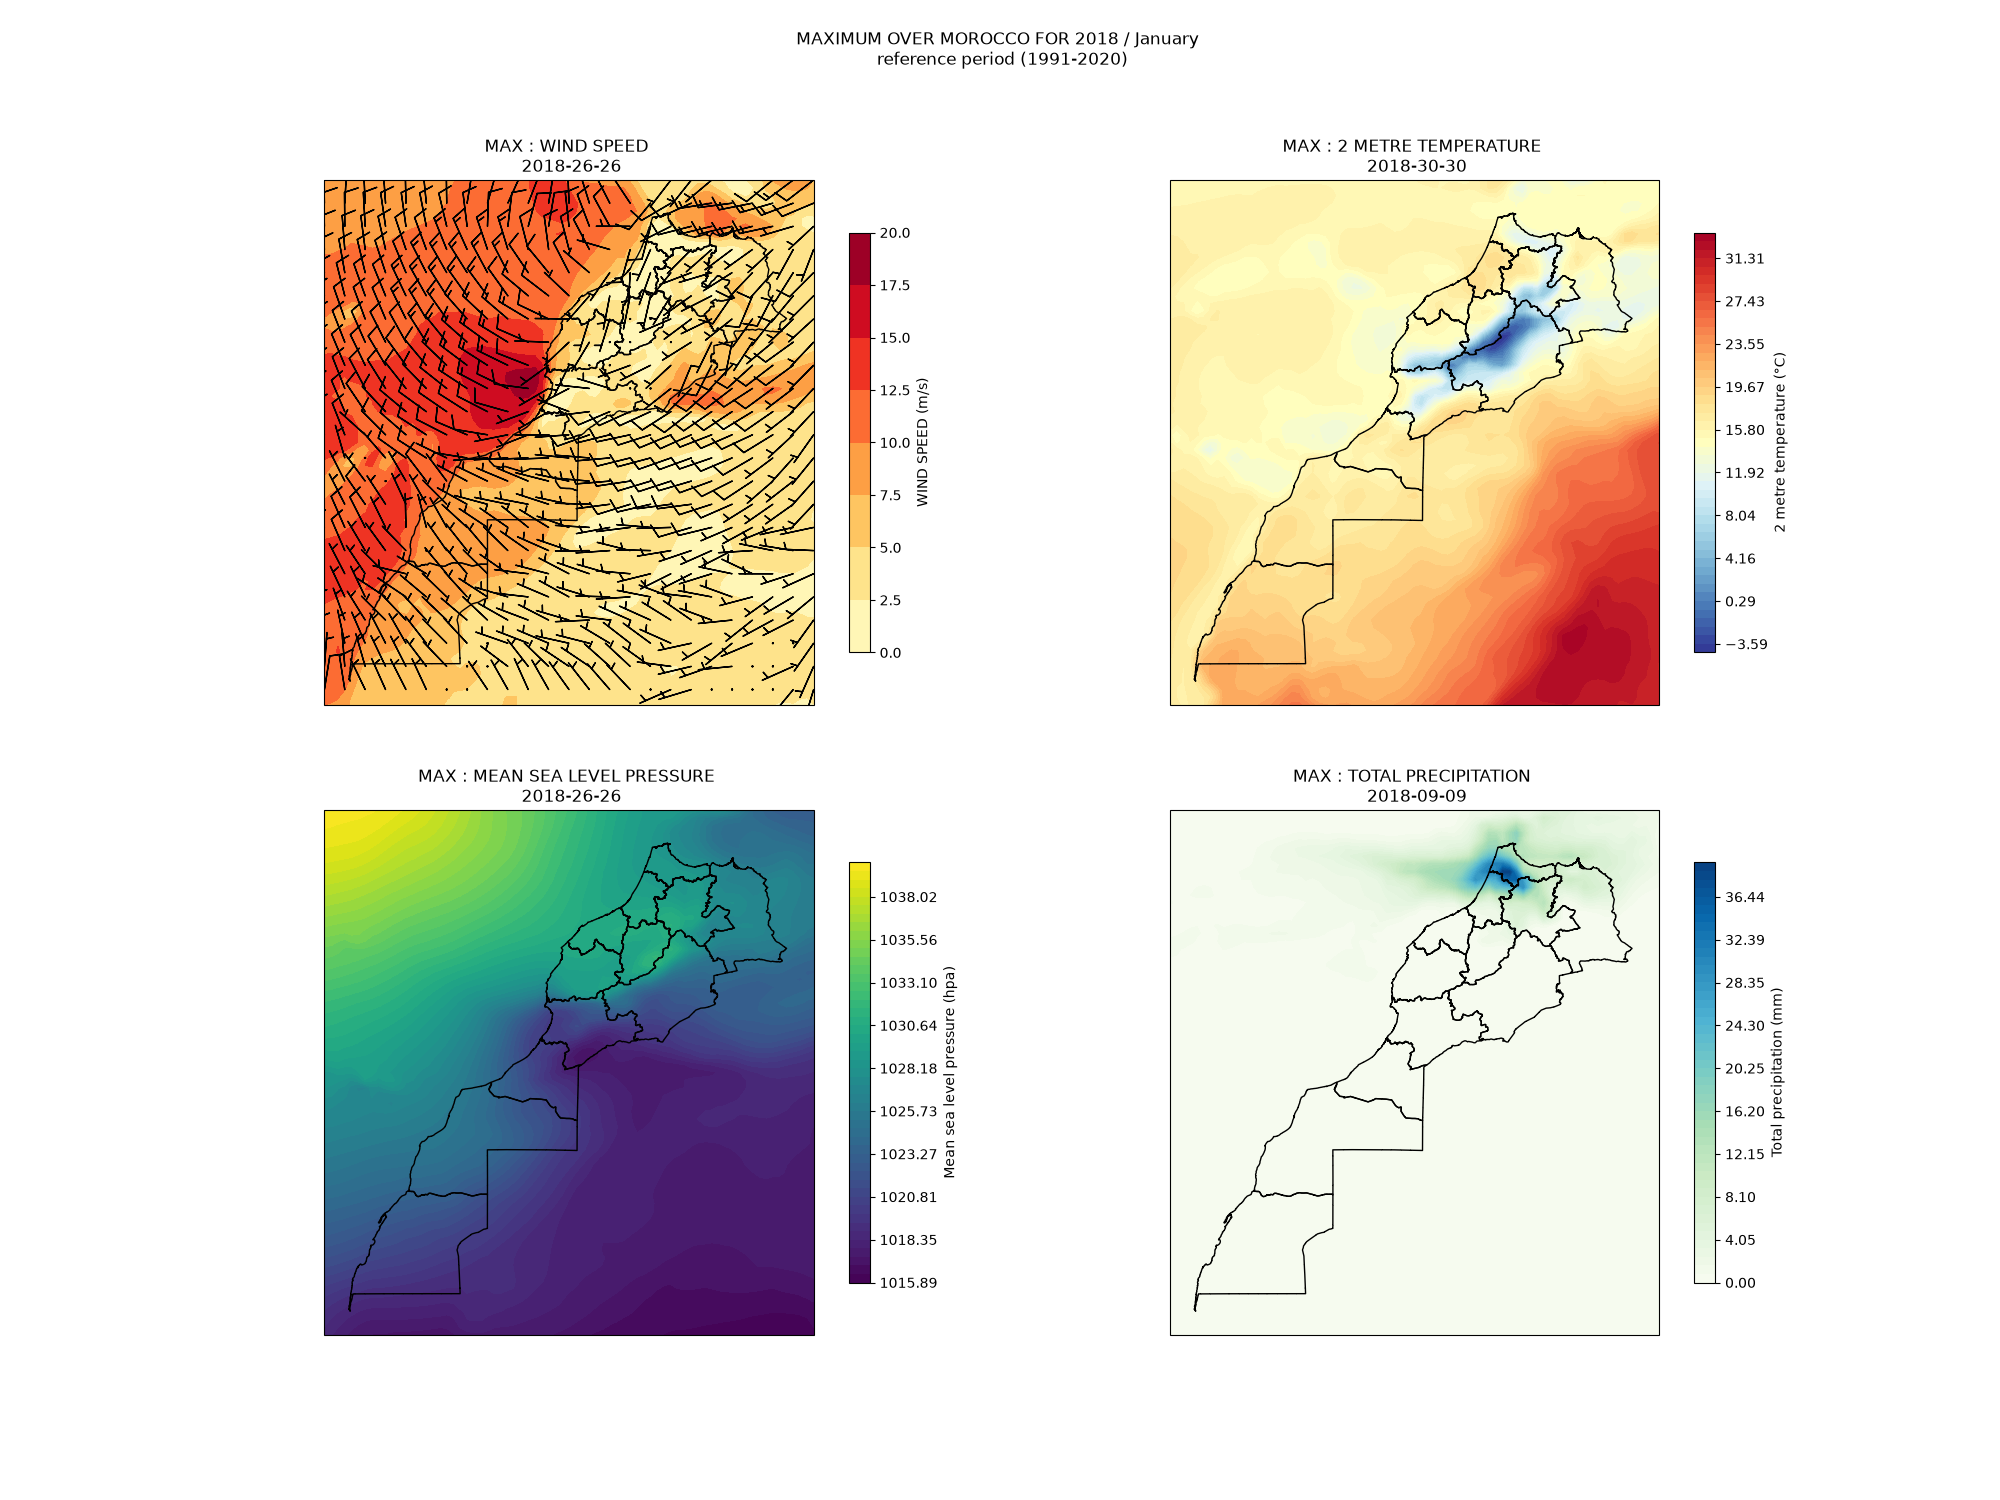
\includegraphics[width=\textwidth]{figures/max_2018_01.png}
    \caption{Valeurs maximales}
\end{figure}

\section{Minimums}

Durant le mois de janvier 2018, les minimums enregistrés pour les différentes variables météorologiques se répartissent ainsi :

* **Température à 2 mètres (t2m) :** La valeur minimale a atteint environ 12,79 °C le 2 janvier 2018 à 15:00, localisée aux coordonnées 32.0°N et -5.75°composante lon.
* **Composante zonale du vent à 10 mètres (u10) :** Un minimum de -2,44 m/s a été relevé le 6 janvier 2018 à 1

\begin{figure}[H]
    \centering
    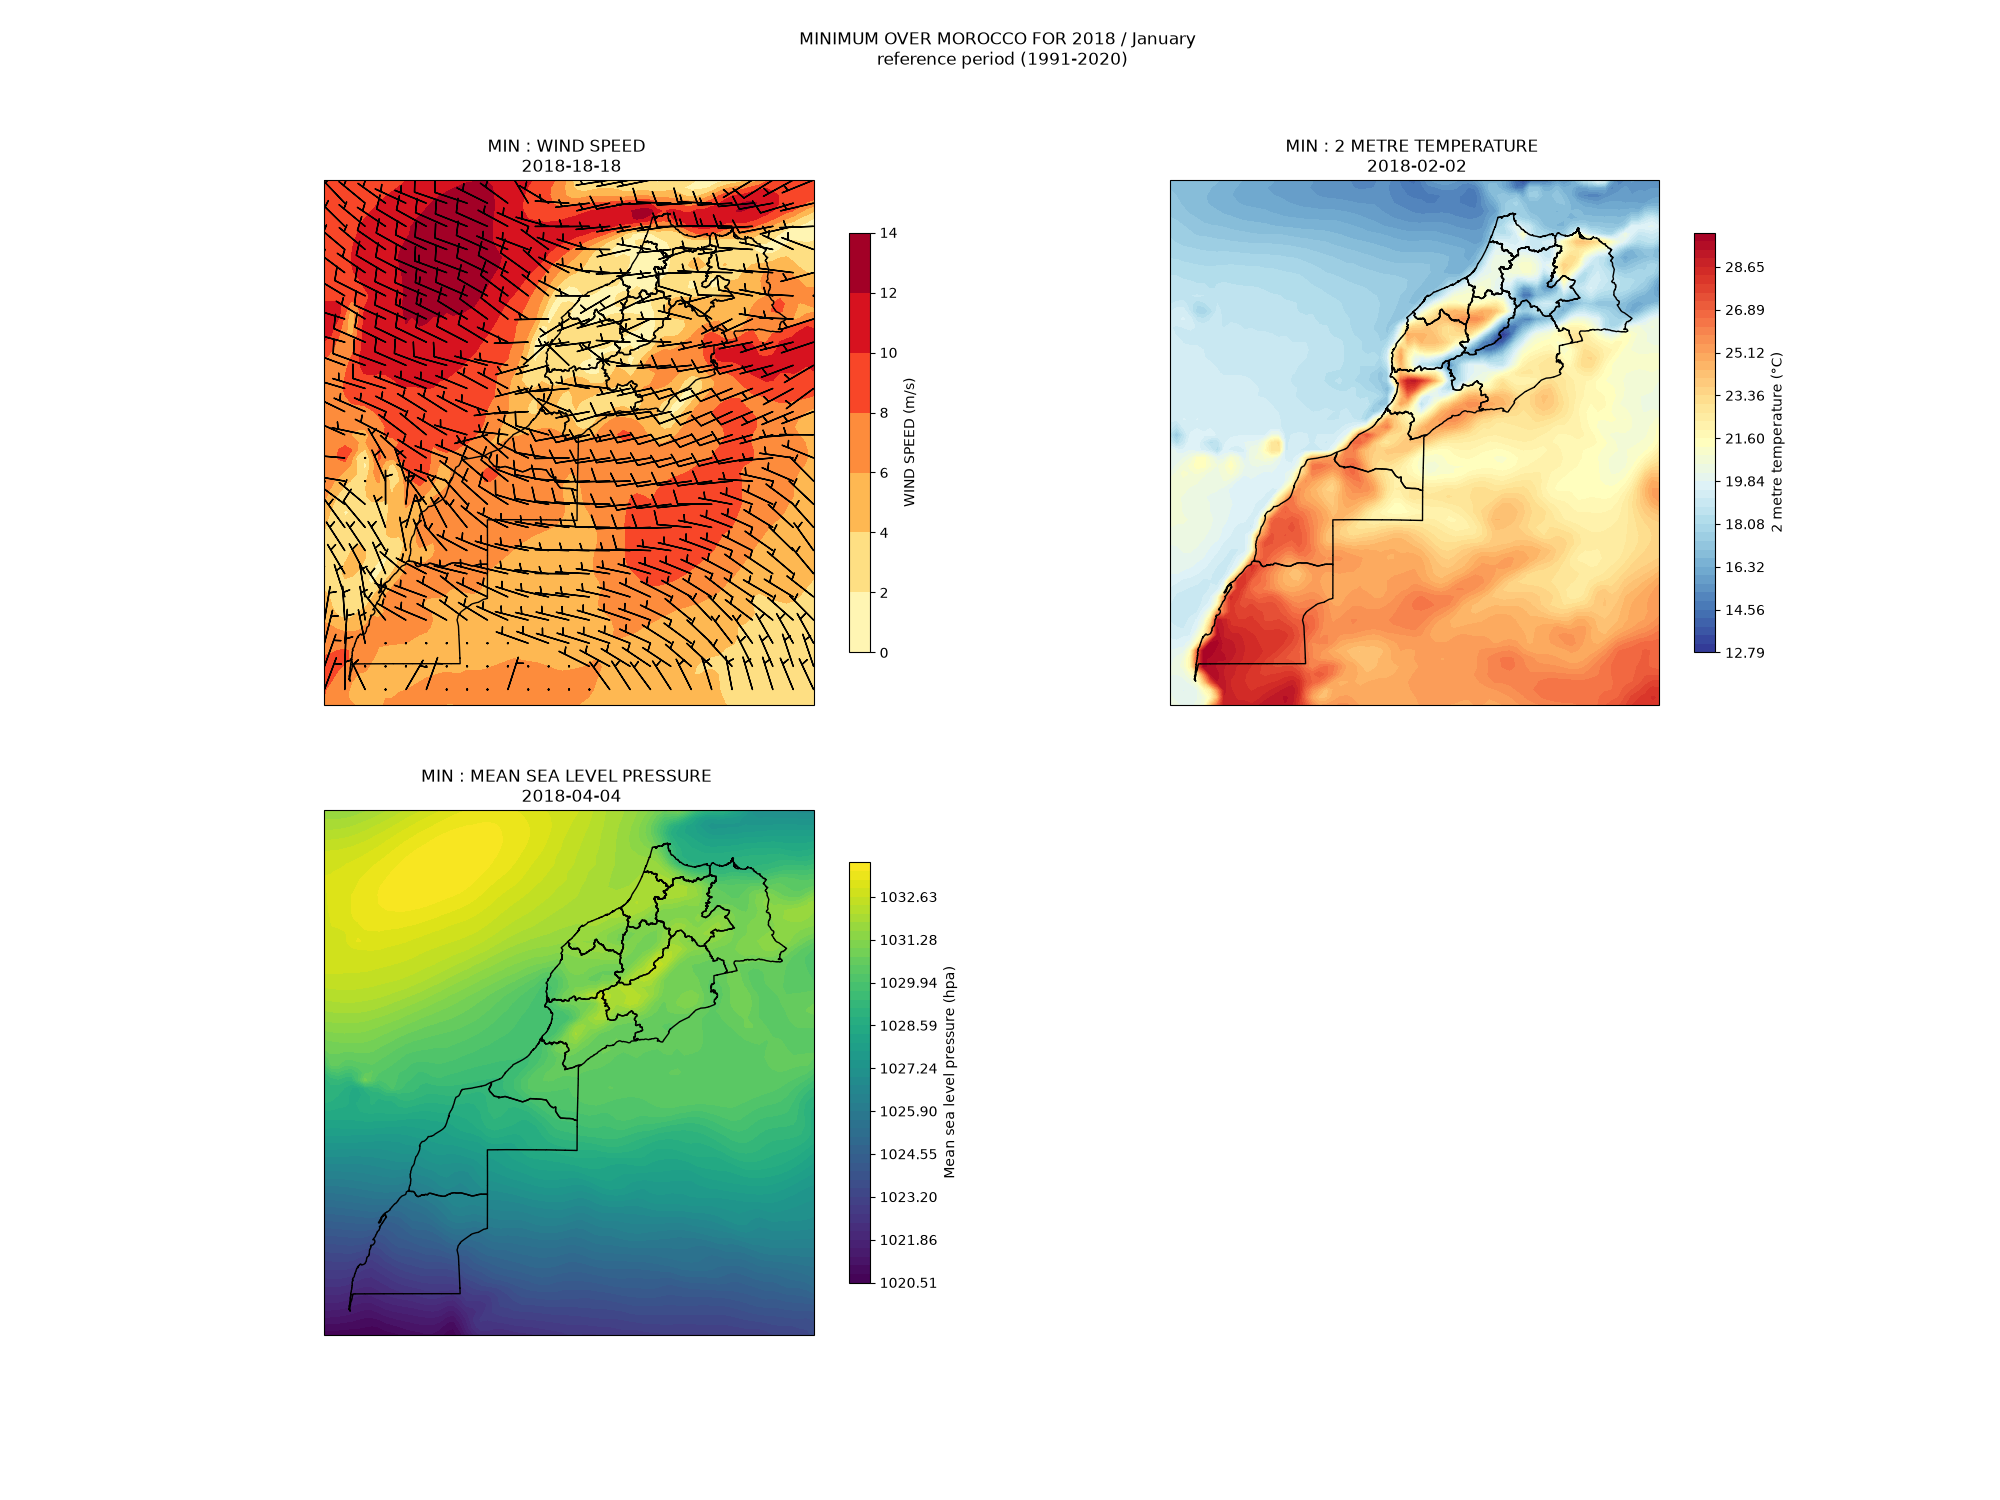
\includegraphics[width=\textwidth]{figures/min_2018_01.png}
    \caption{Valeurs minimales}
\end{figure}

\section{Anomalies}

L'analyse des anomalies climatiques pour le mois de janvier 2018, par rapport à la période de référence 1991-2020, met en évidence une température à 2 mètres (t2m) supérieure à la normale avec une anomalie de +0,41 °C. Durant ce mois, la température maximale de 33,63 °C a été enregistrée le 30 janvier 2018 à 15:00 UTC à la position (22,0°N, -3,25°W), tandis que la température minimale la plus élevée relevée dans le jeu de données a atteint 12,7

\begin{figure}[H]
    \centering
    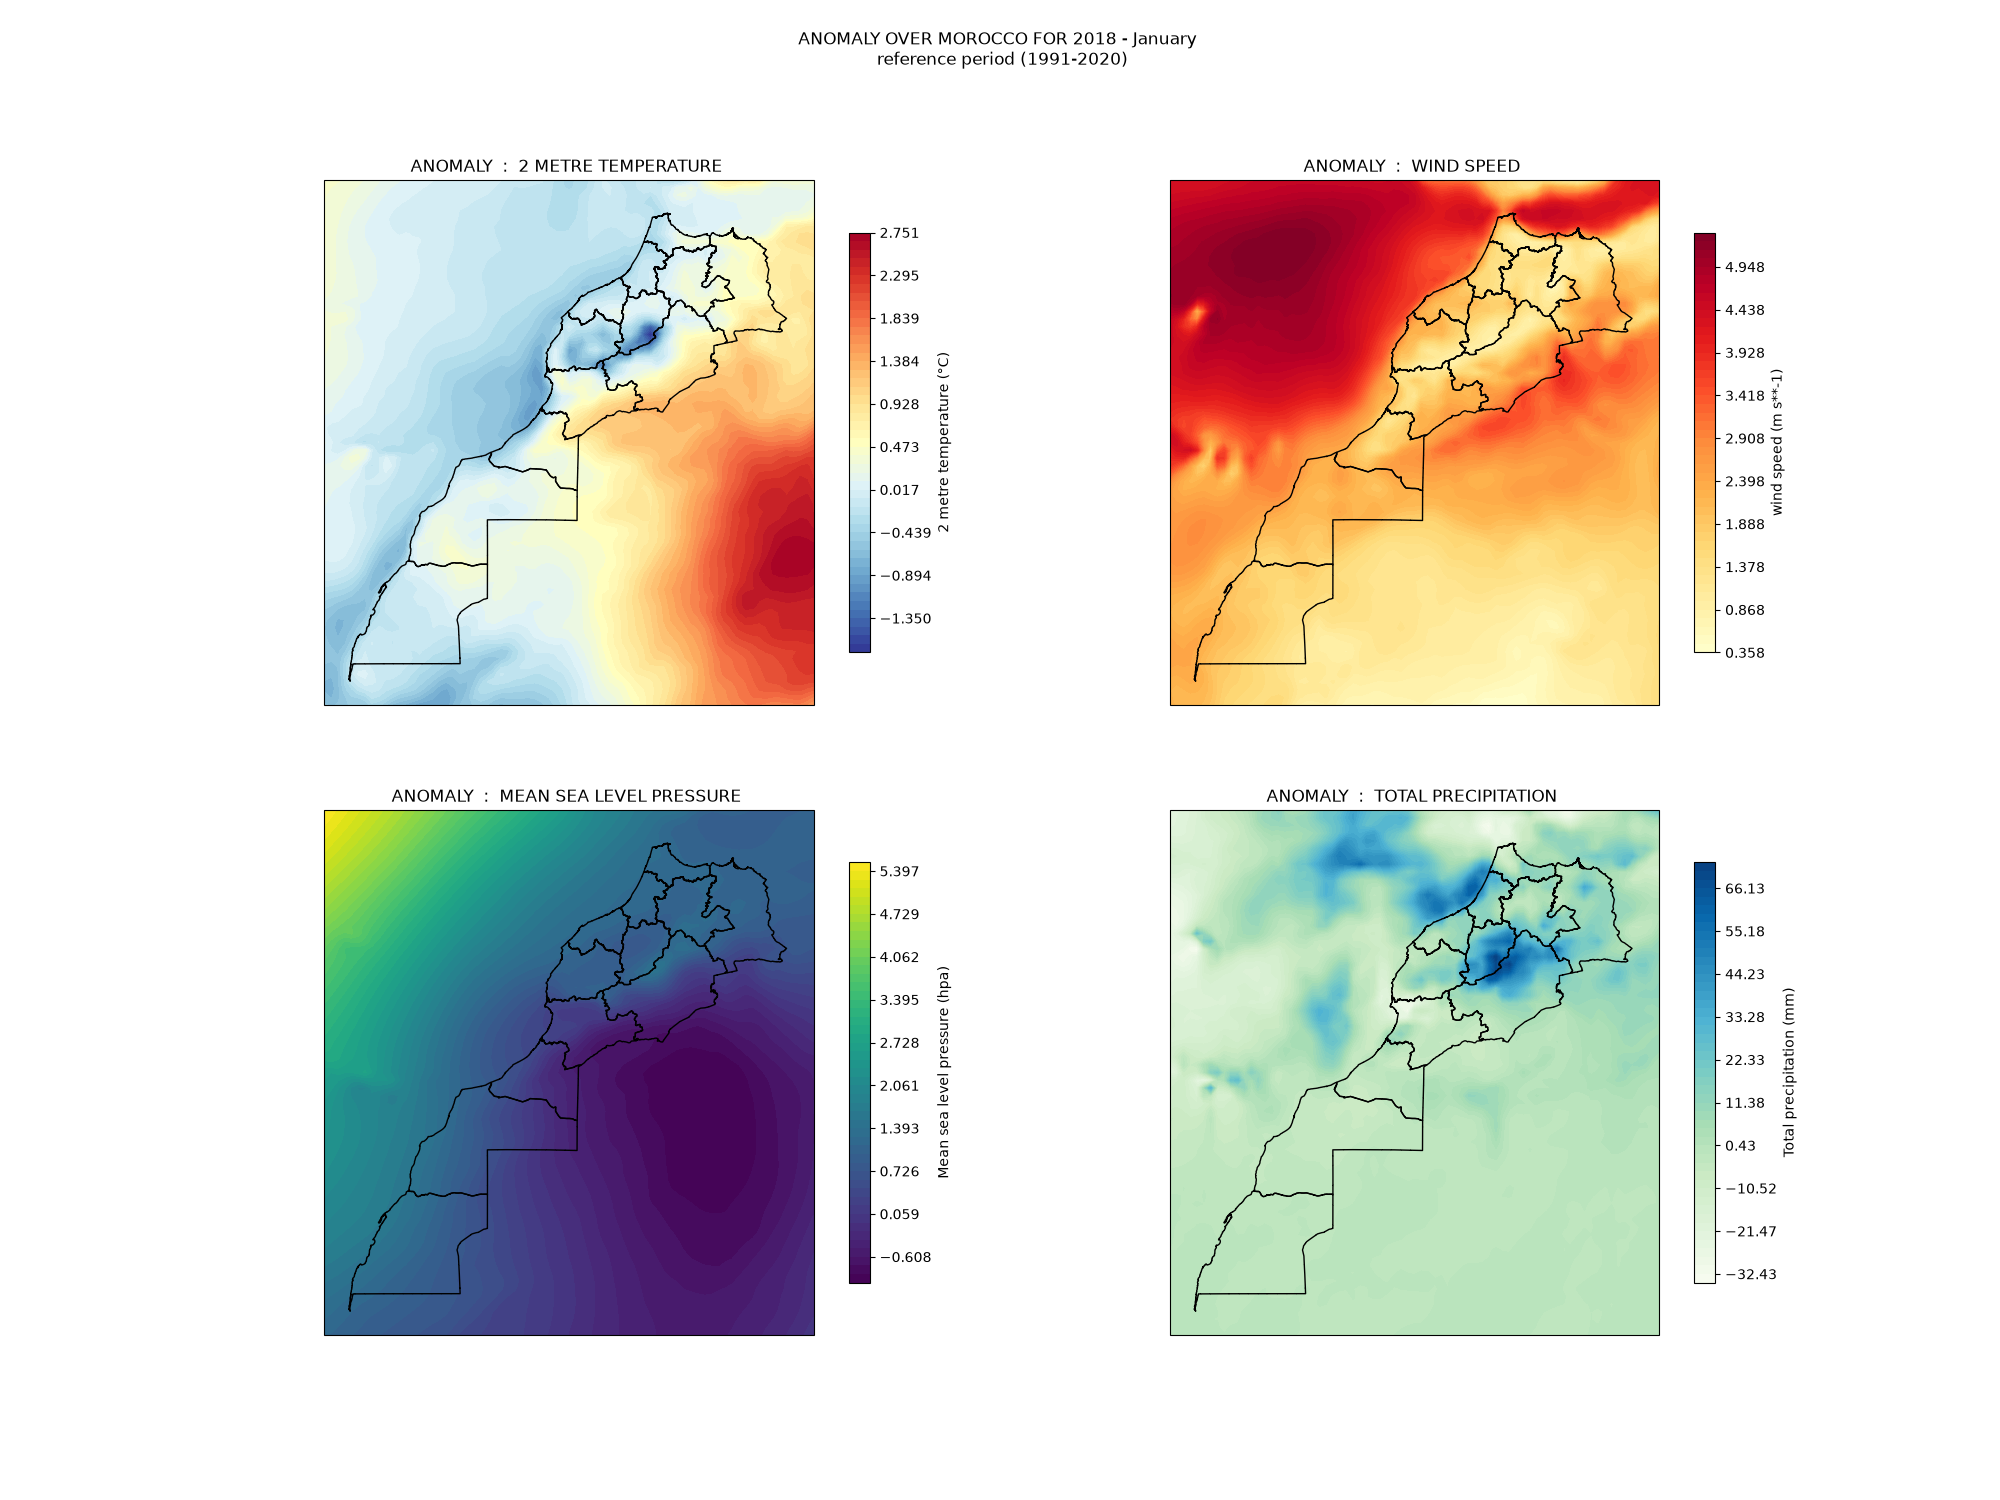
\includegraphics[width=\textwidth]{figures/anom_2018_01.png}
    \caption{Anomalies météorologiques}
\end{figure}

\end{document}
